\section{Einfache FM-Synthese}
\label{einfacheFM}
\FloatBarrier
\subsection{Grundlegende Erläuterungen}
\subsubsection{Auffrischung: Sinus- und Kosinusfunktion mit Parametern}
Die einfachste Form eines Tons lässt sich durch eine Sinus- oder Kosinusschwingung beschreiben. Dabei handelt es sich mathematisch gesehen um eine Sinus- oder eine Kosinusfunktion. Beide gehören zu den \textbf{trigonometrischen Funktionen}, auch \textbf{Winkelfunktionen} genannt. Damit einige später folgende mathematische und für die FM-Synthese erforderliche Rechnungen besser verstanden werden können, wird hier kurz auf die Grundlagen zu Sinus- und Kosinus Funktionen eingegangen. 

Sinus und Kosinus sind \textbf{periodische Funktionen}, d.h. die Funktionswerte wiederholen sich nach einer sogenannten Periode. Mathematisch ausgedrückt muss es dafür eine Konstante $p$  geben, für die bei einem beliebigen x gilt: $\bm{f(x + p) =  f(x)}$ .

Am besten verdeutlichen kann man dies anhand des \textbf{Einheitskreises}. Abbildung \ref{fig:unitcircle} zeigt, wie sich Sinus und Kosinus aus den Seiten eines rechtwinkligen Dreiecks im Einheitskreis berechnen lassen:

\begin{figure} [ht]
\centering
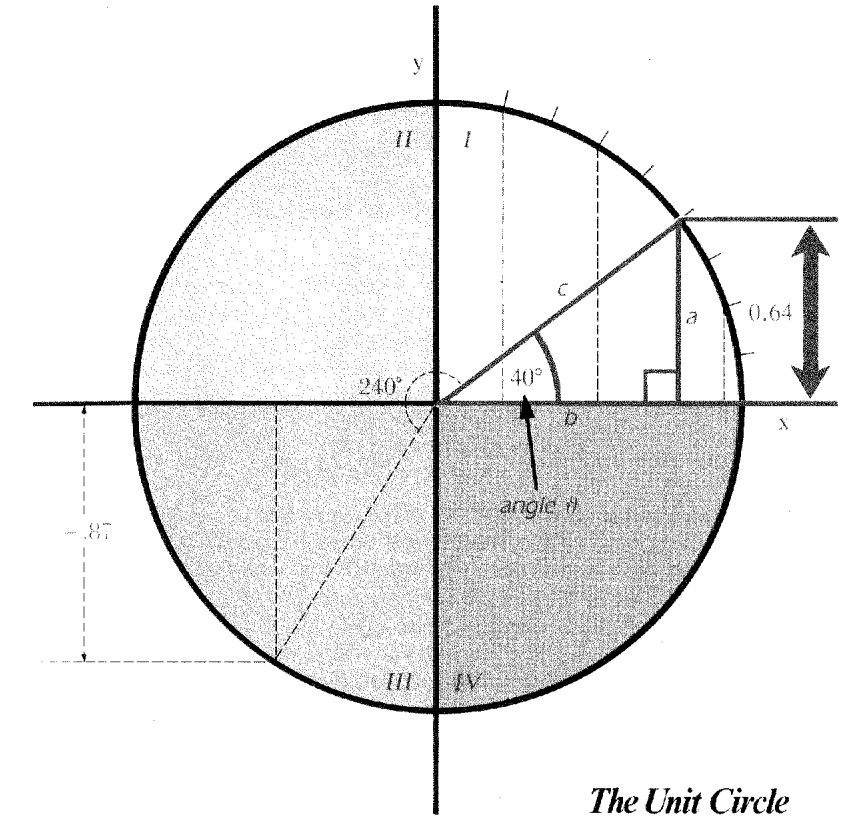
\includegraphics[width=0.7\textwidth]{Unit_Circle.png}
\caption{Der Einheitskreis}
\label{fig:unitcircle}
Quelle: \cite{fmtheory} - Fig. 2.6
\end{figure}

Dabei gilt: 

$\bm{\sin(\theta) = \frac{\textbf{gegenüberliegende Seite}}{\textbf{Hypotenuse}} = \frac{a}{c}}$, wobei die Hypotenuse im Einheitskreis eine Länge von 1 hat. 

$\bm{\to\sin(\theta) = \frac{a}{1} = a}$.

$\bm{\cos(\theta) = \frac{\textbf{anliegende Seite}}{\textbf{Hypotenuse}} = \frac{b}{c} = \frac{b}{1} = b}$ \cite[s. 22 - 27]{fmtheory} \\

\begin{figure} [ht]
\centering
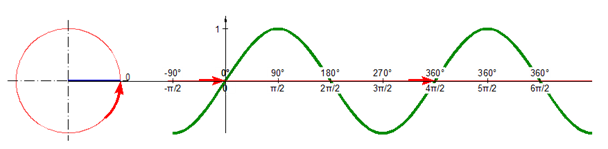
\includegraphics[width=0.95\textwidth]{sinus_einheitskreis.png}
\caption{Vom Einheitskreis zum Sinus}
\label{fig:unitcircleToSinus}
Quelle: \url{http://www.ulrich-rapp.de/stoff/mathematik/Sinus_Einheitskreis.gif}
\\Stand 09.06.2015
\end{figure}

Der aktuelle Winkel im Einheitskreis kann auch im sogenannten \textbf{Bogenmaß} angegeben werden. Das Bogenmaß beschreibt, wie weit der Bogen des Einheitskreises im Uhrzeigersinn abgelaufen wird. Dabei ist $\bm{\pmb{\pi}}$ die sogenannte \textbf{Kreiszahl}. Ein Bogenmaß von $2\pi$ gibt eine ganze Umdrehung im Einheitskreis an, der Wert $\pi$ entspricht einer halben Umdrehung. Um nun auf eine Sinusfunktion überzuleiten, muss das Bogenmaß in Abhängigkeit von der \textbf{Zeit t} angegeben werden, die Formel lautet also dann $\bm{\sin(2\pmb{\pi}*t)}$. Damit festgelegt werden kann, wie oft der Einheitskreis in einer Sekunde abgelaufen wird, multipliziert man das Bogenmaß $2\pi$ mit dem Faktor $\bm{f}$. Dabei entspricht $f$ der \textbf{Frequenz} der Funktion, also wie viele Schwingungen in einer Sekunde durchlaufen werden. Der Wert $\bm{2\pmb{\pi} * f}$ wird auch als \textbf{Kreisfrequenz} bezeichnet.
Man spricht bei Sinus- und Kosinusfunktion auch von Winkelfunktionen, denn man kann den Funktionswert der Funktion auch anhand des Winkels (in Bogenmaß) im Einheitskreis angeben. 
Eine Veranschaulichung des Zusammenhangs zwischen dem Einheitskreis und der Sinusfunktion zeigt Abbildung \ref{fig:unitcircleToSinus}.

Der Unterschied von der Kosinusfunktion zur Sinusfunktion ist, dass der Kosinus bei dem Funktionswert 1 beginnt und Sinus bei Funktionswert 0. Aus diesem Zusammenhang lassen sich folgende Beziehungen (Auch: \textbf{Komplementärformeln}) zwischen Sinus und Kosinus feststellen:\\

\begin{lstlisting}[mathescape]
$\bm{\sin(\frac {\pmb{\pi}}{2} – x) =\cos(x)}$
$\bm{\cos(\frac {\pmb{\pi}}{2} – x) = \sin(x)}$ 
\end{lstlisting}\cite[s. 218]{matheBuch}

Überträgt man diese mathematischen Erkenntnisse nun auf einen Ton, so kann man dessen Funktion wie folgt beschreiben: 		$\bm{y(t) = A * \sin(2 \pmb{\pi} f * t)}$

Um \textbf{90\degree} oder $\bm{\frac{\pmb{\pi}}{2}}$ verschoben gilt: 		$\bm{y(t) = A*\cos(2 \pmb{\pi} f*t)}$

Bei $\bm{A}$ handelt es sich um die \textbf{Amplitude} des Tons, also dessen \textbf{Lautstärke}. Alle Funktionswerte der Funktion werden mit diesem Faktor multipliziert und dadurch größer oder kleiner.

F ist wie oben bereits beschrieben die Frequenz des Tons. Sie gibt die \textbf{Anzahl der Schwingungen (Perioden) pro Sekunde} an und wird in $f=\frac{1}{T}$ angegeben, wobei T die Periodendauer in Sekunden ist. Die Einheit ist Hertz(Hz), also $\frac{1}{s}$.
Je größer die Frequenz eines Tones ist, desto höher klingt er für das Ohr.

Physikalisch gesehen ist ein Ton eine periodische Änderung des Luftdruckt, also Luftmoleküle die um ihre Ruhelage in Schwingung versetzt werden\cite[s. 111 f.]{zwicker}. 

Für das menschliche Ohr hören sich Sinus- und Cosinusschwingungen gleich an, da diese lediglich um $\frac{1}{4}$ der Periode verschoben sind und es in der realen Welt ohnehin keine perfekten Schwingungen geben kann \cite[s. 3f.]{zwicker}. 
\subsubsection{Parameter der FM-Synthese nach Chowning}
\label{chowningparameter}

In diesem Kapitel wird auf die unterschiedlichen Parameter eingegangen, welche in der Formel der einfachen FM-Synthese von John Chowning vorkommen. Zudem wird deren Funktion im Einzelnen beschrieben. Es muss angemerkt werden, dass Chowning in seinen Formeln andere Symbole verwendet als normalerweise in der Nachrichtentechnik üblich. Bei den entsprechenden Symbolen ist eine Anmerkung angefügt.

Die Parameter werden mit der Gleichung in Sinus-Darstellung vorgestellt, d.h. Trägersignal und Modulator sind Sinusfunktionen. Dieselbe Erklärung funktioniert jedoch analog dazu auch mit Cosinus-Funktionen für den Träger und den Modulator.
Die Gleichung für eine frequenzmodulierte Welle lautet wie folgt:
\[ \bm{e(t) = A sin(\pmb{\alpha} t + I sin(\pmb{\beta} t))} \]

\begin{lstlisting}[mathescape]
- $\bm{e(t)} $ beschreibt die [*Amplitude des Modulierten Signals zum Zeitpunkt t*]
- $\bm{A}$ stellt die [*maximale Amplitude des modulierten Signals*] dar
- $\pmb{\alpha} $ ist die [*Kreisfrequenz des Trägersignals*] in $\bm{\frac{1}{s}}$ (Üblich ist hier das Symbol $\omega_c$)
- $\pmb{\beta} $ ist die [*Kreisfrequenz des Modulators*] in $\bm{\frac{1}{s}}$ (Üblich ist hier das Symbol $\omega_m$, $\beta$ wird in der Nachrichtentechnik für den Modulationsindex verwendet)
- $\bm{I}$ stellt den [*Modulationsindex*] dar. Dieser setzt sich wie folgt zusammen: $ \bm{I = \frac{d}{m}} $ mit:
	= [*d: Frequenzhub der Modulation*], d.h. der größte momentane Unterschied zwischen der Frequenz des Trägers und der des modulierten Signals
	Auch: Frequenzänderung, welche durch die Modulation der Trägerfrequenz verursacht wird
	(Hier wird üblicher Weise $\Delta$f als Symbol verwendet)
	=[* m: Kreisfrequenz des Modulators*]
\end{lstlisting} \cite{chowningPaper}

Der Modulationsindex beschreibt also das Verhältnis des Frequenzhubs zur Modulationsfrequenz.
Man kann anhand der Formel bereits erkennen, dass bei einem Modulationsindex von 0 keine Modulation stattfindet. Dabei wird der Frequenzhub der Modulation auch gleich 0, da $ I=\frac{d}{m} $ und somit $ d = 0*m = 0 $ gilt. 
\[ e(t) = A \sin(\alpha t + 0 \sin(\beta t))  \Rightarrow  e(t) = a \sin(\alpha t) \]
Die Frequenz in Hz (Schwingungen pro Sekunde) ergibt sich, wenn man die Kreisfrequenz (siehe oben) durch $2\pi$ teilt.
Anhand der Frequenz des Modulators kann man sehen, wie oft der oben beschriebene Frequenzhub pro Sekunde durchlaufen wird. Beispiel: Bei einer Modulationsfrequenz von 440 Hz wird der Frequenzhub 440 mal pro Sekunde durchlaufen.
